\documentclass[9pt]{IEEEtran}

\usepackage[english]{babel}
\usepackage{graphicx}
\usepackage{epstopdf}
\usepackage{fancyhdr}
\usepackage{amsmath}
\usepackage{amsthm}
\usepackage{amssymb}
\usepackage{url}
\usepackage{array}
\usepackage{textcomp}
\usepackage{listings}
\usepackage{hyperref}
\usepackage{xcolor}
\usepackage{colortbl}
\usepackage{float}
\usepackage{gensymb}
\usepackage{longtable}
\usepackage{supertabular}
\usepackage{multicol}

\usepackage[utf8x]{inputenc}

\usepackage[T1]{fontenc}
\usepackage{lmodern}{}
\input{glyphtounicode}
\pdfgentounicode=1

\graphicspath{{./figures/}}
\DeclareGraphicsExtensions{.pdf,.png,.jpg,.eps}

% correct bad hyphenation here
\hyphenation{op-tical net-works semi-conduc-tor trig-gs}

% ============================================================================================

\title{\vspace{0ex}
MCMC homework}

\author{Marko Medved\vspace{-4.0ex}}

% ============================================================================================

\begin{document}

\maketitle

 \section{Numerical integration vs Monte Carlo integration}
 In this section we compare numerical integration to Monte Carlo integration 
 on a simple domain where the standard numerical integration is possible. Concretly, we approximate 
 the expected value of the (a, b, c)-PERT distribution:

\[
p(x) = \frac{(x - a)^{\alpha - 1} \cdot (c - x)^{\beta - 1}}{\mathrm{B}(\alpha, \beta) \cdot (c - a)^{\alpha + \beta - 1}}
\]
 with a = 0, b = 10 and c = 100. 


 \subsection{Trapezoidal rule}
We begin by approximating the expected value using the Trapezoidal rule.
 To determine how many function evaluations are required, we first
  computed the exact expected value analytically: 
  $\mathbb{E}[X] = 23.\overline{3}$. We then applied the numerical method,
   incrementally increasing the number of function evaluations until the
    result was accurate to four decimal places (the difference between estimated 
    and true value was less that $5 \times 10^{-5}$). This level of precision was 
    achieved with 271 evaluations.

 \subsection{CLT estimation for Monte-Carlo}
In this section, we estimate the expected value using Monte Carlo integration.
 Our objective is to determine how many random samples are needed to approximate
  the integral within two decimal places, with 95\% confidence.
 
The Monte-Carlo approximation in this example is done by drawing
 independent samples
  \( x_1, x_2, \dots, x_n \sim \mathcal{U}(a, c) = \mathcal{U}(0, 100) \), and estimating:

\[
\mathbb{E}[X] = \int_a^c x \cdot p(x) \, dx \approx \frac{c - a}{n} \sum_{i=1}^n x_i p(x_i).
\]

Let this estimator be denoted by \( \hat{\mu}_n \). By the Central Limit Theorem, the standard error of \( \hat{\mu}_n \) is approximately:

\[
SE = \frac{\hat{\sigma}}{\sqrt{n}},
\]

where \( \hat{\sigma}^2 \) is the sample variance of the integrand values \( x_i p(x_i) \).

To estimate \( \mathbb{E}[X] \) to 2 decimal places with 95\% confidence, we require:

\[
1.96 \cdot \frac{\hat{\sigma}}{\sqrt{n}} \leq 0.005.
\]

So to estimate the number of points, we need to compute $\sigma$. Since this 
is the variance of our integrand, we decided to estimate it using a pilot run
 of $10^8$ samples. Our estimation was $\hat{\sigma} = 19.08$ and then we calculated: 
 $n \approx 55935632$. 



 \subsection{Numerical samples verification}
To verify our estimate of the required number of samples, we perform 
200 independent Monte Carlo simulations. We then compute the difference 
between each estimate and the true expected value, and visualize
 the distribution of these differences as a density plot in 
 Figure~\ref{fig:diff}. We can see that almost all samples, as expected since we defined the 
 95\% confidence, have an absolute 
 difference to the true value less than 0.005. We can also seee that the density is gathered 
 around 0. 

    \begin{figure}[h]
        \centering
        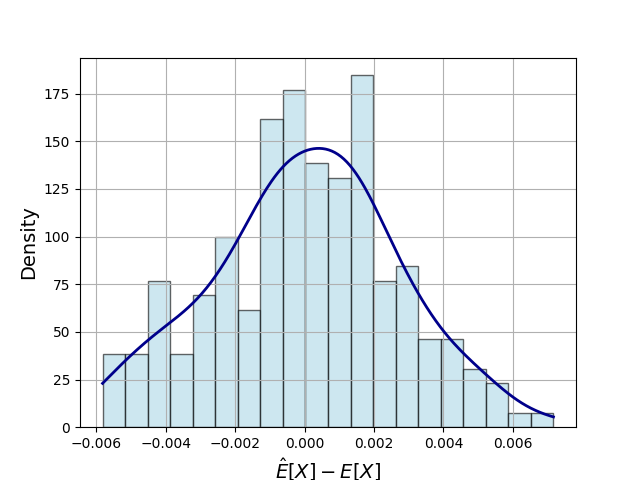
\includegraphics[width=0.99\columnwidth]{figures/diff.png}
        \caption{Density of differences of the estimated and true expected value}
        \label{fig:diff}
    \end{figure}



 \subsection{Comparison of results from both methods}
As expected, the trapezoidal rule significantly outperformed the Monte Carlo
 method. It provided a deterministic result accurate to four decimal places 
 using relatively few evaluations, while the Monte Carlo estimate required 
 many more samples and achieved only two-decimal-place accuracy with 95\%
  confidence. This highlights that for low-dimensional problems with simple
   domains, standard numerical integration methods are preferable to Monte 
   Carlo methods.

\section{Importance sampling}
In this section we implement importance sampling for Monte Carlo integration
 on the provided integral:
 $I = \int_0^1 x^{-3/4} \cdot e^{-x} \, dx$

We plot the integrand ($f(x) = x^{-3/4} \cdot e^{-x}$) on Figure\ref{fig:lin}. We can see that 
the bulk of the integral is gathered really close to 0.


    \begin{figure}[h]
        \centering
        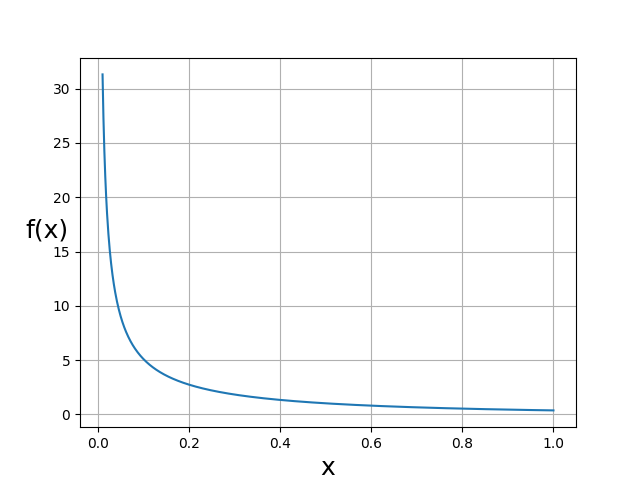
\includegraphics[width=0.99\columnwidth]{figures/f}
        \caption{Graph of the given function}
        \label{fig:lin}
    \end{figure}

 \subsection{Uniform distribution}
 Here we use the uniform distribution as the distribution we want to sample from.
 Since our uniform distribution is from 0 to 1, the estimation of the integral is
 simply: 
 \[
I \approx \frac{1}{n} \sum_{i=1}^{n} f(x_i)
\]
As we have seen on Figure~\ref{fig:lin}, the function has a shape that is very concentrated at 
0 so the uniform choice might not be the best. 

 \subsection{The provided distribution}
 Next we use the provided distribution ($q(x) = c \times x^{-3/4}$).
 
 Firstly, we determine the $c$ constant to be $1/4$ so that the distribution
  integrates to 1 over the domain $[0, 1]$. 

 Next, to implement inversion sampling, we need the CDF and it's inverse. 
 We calculated these functions to be: 
\begin{align*}
F(x) &= x^{1/4} \\
F^{-1}(x) &= x^4
\end{align*}
Then we simply sampled from the uniform distribution on the $[0, 1]$ interval, 
and transormed those samples with our inverse CDF to get the samples of $q(x)$.

Lastly, we implemented the importance sampling. Our integral can now be approximated as:
\[
I \approx \frac{1}{n} \sum_{i=1}^{n} \frac{f(x_i)}{ q(x_i)}
\] 


 \subsection{Comparison of results from both methods}
Here we compare the results of two Monte Carlo integration methods. For each method, we drew 10 independent 
samples of size$n = 10^7$, computed the average estimate, and calculated the corresponding
 standard deviation. The results are summarized in Table~\ref{tab:imp}.  

\begin{table}[h]
    \centering
    \begin{tabular}{c|c|c}

    \textbf{Sampling Distribution} & \textbf{Estimate} & \textbf{Standard Deviation} \\
    \hline
    Uniform  & 3.3640 & 0.0890 \\
    $q(x)$ & 3.3795 & 0.0001 \\
    \end{tabular}
    \caption{Comparison of Importance Sampling Estimates}
    \label{tab:imp}
\end{table}

As shown in the table, using $q(x)$ as a proposal distribution results in a significantly 
lower standard deviation compared to uniform sampling. This improvement is expected, as
$q(x)$ closely matches the shape of the integrand, leading to more samples being drawn
 from regions that contribute most to the integral. Consequently, the variance of the 
 estimator is greatly reduced.

\section{Metropolis-Hastings algorithm}
Here, we implement the Metropolis-Hastings algorithm to compute the mean and 
the variance of the $\eta$ and $\alpha$, which are the parameters of the Weibull 
distribution which is the distribution of our random variable. 

Firstly, we compute the posterior from the given likelihood and prior: 
\[
p(\alpha, \eta | x) \propto \left( \prod_{i=1}^{n} \alpha \, \eta \, x_i^{\alpha - 1} \, e^{-\eta x_i^\alpha} \right) \cdot e^{-\alpha - 2 \eta} \, \eta
\]




        

\end{document}
